%% IEEE Transactions submission version (standard IEEEtran journal style,
%% not the Computer Society variant).
%%
%% Formatted to the constraints in IEEE/README.md: double column, 10pt,
%% <= 8 pages (the no-fee ceiling under the traditional access model),
%% abstract <= 250 words in a single paragraph with no citations, equations or
%% undefined abbreviations, and no author biographies.
%%
%% Build:  make -C IEEE        (figures, tables and macros come from ../paper)
\documentclass[10pt,journal]{IEEEtran}

\usepackage{cite}
\usepackage{amsmath,amssymb}
\usepackage{graphicx}
\usepackage{booktabs}
\usepackage{tikz}
\usepackage{xcolor}
\usepackage{url}
\usepackage[hidelinks,breaklinks]{hyperref}

\usetikzlibrary{arrows.meta,positioning}

% Experimental values, generated by ../paper/experiments.py.
% Generated by paper/experiments.py -- do not edit by hand.
% 2026-09-22T17:52:14+00:00

\newcommand{\expNumSeeds}{20}
\newcommand{\expSimHours}{24}
\newcommand{\expEventsTotal}{3584}
\newcommand{\expBenignEvents}{3111}
\newcommand{\expTelemetryEvents}{2880}
\newcommand{\expCommandEvents}{583}
\newcommand{\expAuditEvents}{102}
\newcommand{\expDownlinkEvents}{19}
\newcommand{\expPrecision}{0.997}
\newcommand{\expPrecisionSD}{0.002}
\newcommand{\expFprOverall}{0.06}
\newcommand{\expFindingsMean}{613}
\newcommand{\expAucMulti}{0.996}
\newcommand{\expAucMultiSD}{0.001}
\newcommand{\expAucUni}{0.998}
\newcommand{\expAucUniSD}{0.000}
\newcommand{\expLeadMean}{42}
\newcommand{\expLeadSD}{2}
\newcommand{\expLeadMin}{37}
\newcommand{\expLeadMax}{44}
\newcommand{\expThroughputRules}{189\,012}
\newcommand{\expThroughputMl}{78\,880}
\newcommand{\expUsPerEventMl}{12.7}
\newcommand{\expFitSeconds}{0.02}
\newcommand{\expModelKb}{1.5}
\newcommand{\expRuleCount}{21}
\newcommand{\expAucSwapMulti}{0.322}
\newcommand{\expAucSwapMultiSD}{0.026}
\newcommand{\expAucSwapUni}{0.385}
\newcommand{\expAucSwapUniSD}{0.019}
\newcommand{\expSwapDetectedMulti}{1}
\newcommand{\expSwapDetectedUni}{1}
\newcommand{\expSwapMedianNormal}{4.6}
\newcommand{\expSwapMedianSwapped}{2.9}
\newcommand{\expSwapWindowMin}{50}
\newcommand{\expAucBaselineMin}{0.974}
\newcommand{\expAucBaselineMax}{0.994}
\newcommand{\expRecAnomalyRules}{0.19}
\newcommand{\expMttdAnomalyRules}{47}
\newcommand{\expMttdAnomalyAll}{6}
\newcommand{\expPrecisionRules}{0.991}
\newcommand{\expPrecisionMl}{1.000}
\newcommand{\expFprOneHour}{77}
\newcommand{\expFprFullDay}{0.2}
\newcommand{\expFprTelemetryOp}{0.2}
\newcommand{\expAlertPeakHour}{176}
\newcommand{\expCriticalPerDay}{26}
\newcommand{\expFpAuthPerTrial}{1.00}
\newcommand{\expFpRatePerTrial}{1.58}
\newcommand{\expRecCredentialCompromise}{0.82}
\newcommand{\expRecSDCredentialCompromise}{0.00}
\newcommand{\expDetCredentialCompromise}{100}
\newcommand{\expMttdCredentialCompromise}{18}
\newcommand{\expRecCommandTampering}{1.00}
\newcommand{\expRecSDCommandTampering}{0.00}
\newcommand{\expDetCommandTampering}{100}
\newcommand{\expMttdCommandTampering}{0}
\newcommand{\expRecReplay}{1.00}
\newcommand{\expRecSDReplay}{0.00}
\newcommand{\expDetReplay}{100}
\newcommand{\expMttdReplay}{0}
\newcommand{\expRecAnomalousBehavior}{0.97}
\newcommand{\expRecSDAnomalousBehavior}{0.00}
\newcommand{\expDetAnomalousBehavior}{100}
\newcommand{\expMttdAnomalousBehavior}{342}
\newcommand{\expRecExfiltration}{1.00}
\newcommand{\expRecSDExfiltration}{0.00}
\newcommand{\expDetExfiltration}{100}
\newcommand{\expMttdExfiltration}{0}

\graphicspath{{figures/}}

\definecolor{vizblue}{HTML}{2A78D6}
\definecolor{vizorange}{HTML}{EB6834}
\definecolor{vizaqua}{HTML}{1BAF7A}
\definecolor{vizink}{HTML}{52514E}

\begin{document}

\title{Cloud-Native Detection of Cyberattacks Against Satellite Ground
Stations: An Open, Labelled Testbed and Two Negative Results}

% TODO before submission: full name, affiliation, and e-mail of each author.
\author{Henrique~[Surname]%
\thanks{The author is an independent researcher. Code, data and the experiment
harness: \url{https://github.com/rikosoo/Cloud-Native-Detection-of-Cyberattacks-Against-Satellite-Ground-Stations}.}}

\markboth{IEEE Transactions (submitted)}%
{Henrique: Cloud-Native Detection of Cyberattacks Against Satellite Ground Stations}

\IEEEtitleabstractindextext{%
\begin{abstract}
The space segment of a satellite mission is expensive to reach; the ground
segment that commands it is an ordinary cloud workload with operators,
credentials and object storage. Published satellite-security research
concentrates on the spacecraft and the radio link, and no labelled corpus
exists for measuring ground-segment detection. We present an open testbed: a
simulated ground station emitting four correlated planes of evidence, five
adversary-emulation scenarios with per-event ground truth, and a cloud-native
pipeline of \expRuleCount{} stateful rules plus an unsupervised telemetry
baseline. Over \expNumSeeds{} independent \expSimHours-hour trials it detects
all five scenarios in every trial at a precision of \expPrecision{}, flagging
\expFprOverall\% of benign events. The learned baseline makes a sub-threshold
behavioural drift visible \expLeadMean{} minutes before the first spacecraft
limit violation, raising event-level recall for that scenario from
\expRecAnomalyRules{} to \expRecAnomalousBehavior{}. Two results contradict our
design rationale. First, the multivariate model does not outperform a
well-calibrated per-channel detector on that drift: areas under the receiver
operating characteristic curve are \expAucMulti{} and \expAucUni{}. Second, a
probe that preserves every marginal distribution while destroying the joint
structure, by replaying housekeeping frames from half an orbit earlier, is
invisible to both detectors, scoring \expAucSwapMulti{} and \expAucSwapUni{}
and alerting in \expSwapDetectedMulti{} of \expNumSeeds{} trials, because a
baseline fitted over a whole orbit marginalises away the phase information the
attack violates. Fitting that baseline on less than one full diurnal cycle also
raises the telemetry false-positive rate from \expFprFullDay\% to
\expFprOneHour\%. All code and data are public.
\end{abstract}

\begin{IEEEkeywords}
Satellite ground stations, space systems security, intrusion detection, anomaly
detection, cloud computing security, adversary emulation, telemetry.
\end{IEEEkeywords}}

\maketitle
\IEEEdisplaynontitleabstractindextext
\IEEEpeerreviewmaketitle

\section{Introduction}

\IEEEPARstart{A}{satellite} is difficult to attack directly and difficult to
repair once attacked. The ground station that commands it is neither. Modern
ground segments are built from the same components as any other cloud workload:
identity providers, application programming interfaces, message queues, object
storage and the operators who hold the credentials. An adversary who reaches the
commanding path from there inherits authority over the vehicle without ever
touching a radio.

Recent work has made the space segment measurable. Willbold et
al.~\cite{willbold2023space} performed the first systematic software-security
analysis of real satellite firmware; Pavur et al.\ demonstrated large-scale
interception of operational satellite links~\cite{pavur2020vsat} and argued for
a research agenda built on reproducible artefacts~\cite{pavur2020sok}. Policy
has followed, with Space Policy Directive-5 naming the ground segment
explicitly as part of the protected system~\cite{spd5}, and the community now
has a space-specific adversary taxonomy in SPARTA~\cite{sparta}.

What is missing is the thing that made progress possible in network intrusion
detection: an open corpus with ground truth. Surveys of network intrusion
detection datasets list dozens of options~\cite{ring2019datasets}; for the
satellite ground segment there is, to our knowledge, none. Ground-segment
telemetry and audit logs are operationally sensitive and rarely published, and
when they are, they are unlabelled. The practical consequence is that
ground-segment detection claims cannot be compared, and that a detector's cost
--- in false positives, in analyst time, in compute --- is usually not reported.

This paper contributes a testbed and an evaluation rather than a new detector:

\begin{itemize}
  \item \textbf{An open, labelled ground-station corpus generator}
  (Section~\ref{sec:impl}). A simulated station emits four correlated planes of
  evidence, and five adversary-emulation scenarios inject themselves into that
  timeline, labelling every event they create or modify. Scenarios compose: the
  stolen session established by the credential stage is the one the tampering
  and exfiltration stages reuse.
  \item \textbf{A cloud-native detection pipeline} (Section~\ref{sec:design}).
  \expRuleCount{} stateful rules covering identity, commanding integrity,
  replay, spacecraft limits and exfiltration, each mapped to an ATT\&CK
  technique~\cite{attack} and emitted in a standard finding
  format~\cite{asff}, plus an unsupervised telemetry baseline that runs inside
  a serverless function with no machine-learning runtime.
  \item \textbf{A measured evaluation with negative results}
  (Sections~\ref{sec:method}--\ref{sec:results}). Twenty independent trials, an
  ablation separating rules from the model, comparisons against the two
  alternatives a real mission already has, a probe that isolates joint
  structure from marginals, a baseline-size sweep, and the compute cost. Two
  findings contradict the rationale we designed the model around, and we report
  them as such.
\end{itemize}

We organise the evaluation around five questions. \textbf{RQ1:} does the
pipeline detect each scenario, and at what precision? \textbf{RQ2:} what does
the learned baseline add over the spacecraft's own limit checks, the
alternative a real mission already operates? \textbf{RQ3:} does the
multivariate model add anything over a well-calibrated per-channel detector?
\textbf{RQ4:} how much clean telemetry does the baseline need before it is
usable? \textbf{RQ5:} what does the pipeline cost to run?

\section{Background and Threat Model}
\label{sec:background}

\subsection{The ground segment as an attack surface}

A ground station converts operator intent into authenticated telecommands and
spacecraft state into archived data products. Four kinds of record are
produced, and a detector needs all four: \emph{telemetry} (spacecraft
housekeeping --- bus voltage and current, battery state of charge, amplifier
and battery temperatures, link margin --- downlinked during a contact);
\emph{telecommands} (CCSDS telecommand frames~\cite{ccsds232}, authenticated in
modern missions by the Space Data Link Security protocol~\cite{ccsds355}, which
supplies a keyed authentication tag and an anti-replay sequence counter);
\emph{cloud audit records} (who signed in, from where, with what authenticator,
and which interfaces they called); and \emph{downlink transfers} (payload
products moving into, and potentially out of, the mission archive).

The first two describe the vehicle; the last two describe the enterprise. Most
published space-security work addresses the first two, and most enterprise
security tooling addresses the last two. An intrusion crosses between them,
which is the observation the design in Section~\ref{sec:design} is built on.

\subsection{Adversaries and trust boundaries}

We consider three profiles, following~\cite{manulis2021newspace}
and~\cite{falco2019principles}: the \emph{opportunistic} adversary, commodity
tooling and no mission knowledge, high volume and low stealth; the
\emph{insider}, a badged operator acting outside their role with legitimate
credentials from legitimate networks at legitimate times, so that only
\emph{what} they do is anomalous and every network- and identity-provenance
rule is defeated by construction; and the \emph{state-sponsored} adversary,
patient and mission-aware, who targets key material and the commanding path,
disables logging early, and prefers degradation indistinguishable from a bus
fault, because an operator who believes the spacecraft is unhealthy will act on
the wrong runbook.

Four boundaries separate the operator from the vehicle: the human-to-cloud
boundary (B1, defended by multi-factor authentication and network policy), the
cloud control plane (B2, least-privilege authorisation and audit logging), the
uplink (B3, the authentication tag and sequence counter) and the spacecraft
itself (B4, on-board limit checks). Table~\ref{tab:paths} maps the five attack paths we emulate to
SPARTA~\cite{sparta} and ATT\&CK~\cite{attack}. Briefly:
\texttt{credential\_compromise} sprays passwords, signs in without
multi-factor authentication from an untrusted netblock outside duty hours,
creates an access key, attaches an administrative policy and deletes the audit
trail; \texttt{command\_tampering} rewrites opcodes and parameters in flight,
forges an authentication tag with the wrong key, issues an out-of-role command
and floods the uplink; \texttt{replay} retransmits recorded frames verbatim
hours later, where the tag still verifies because the adversary never held the
key~\cite{syverson1994replay}; \texttt{anomalous\_behavior} commands a
degradation in which every channel stays inside its interface-control limits
while the relationships between them break; and \texttt{exfiltration}
enumerates the archive, reads objects in bulk and copies multiple gigabytes
cross-account to an unapproved destination.

\begin{table}[t]
\caption{Emulated attack paths and framework mapping. B1--B4 are the trust
boundaries defined above; the ATT\&CK column gives the primary technique.}
\label{tab:paths}
\centering
\footnotesize
\begin{tabular}{@{}llll@{}}
\toprule
\textbf{Scenario} & \textbf{Bnd.} & \textbf{SPARTA} & \textbf{ATT\&CK} \\
\midrule
Credential compromise & B1, B2 & IA-0004 & T1078.004 \\
Command tampering & B3 & EX-0012 & T1565.002 \\
Replay & B3 & EX-0013 & T1557 \\
Anomalous behaviour & B4 & IMP-0002 & T1565.001 \\
Exfiltration & B2 & EXF-0003 & T1537 \\
\bottomrule
\end{tabular}
\end{table}

We assume the event stream reaches the detector: an adversary who can silently
suppress telemetry defeats every rule, which is why the deployed pipeline alarms
on the \emph{absence} of events. We assume audit logging is on, and treat its
disabling as itself a critical finding. We assume telecommand key material is
not already stolen; when it is, the integrity rule goes quiet and only the
behavioural rules remain, which is why the catalogue does not rest on the
authentication tag alone.

\section{System Design}
\label{sec:design}

Figure~\ref{fig:arch} shows the pipeline. Three properties drove the design.
\emph{One engine, three runtimes}: the detection engine imports no cloud
software development kit, and runs unchanged in the offline command-line tool,
in the test suite, and inside a serverless function; cloud services are reached
only through an event sink interface and a state-store interface.
\emph{Offline first}: the full pipeline --- generate, fit, detect, score ---
runs with a numerical library and a configuration parser, with no credentials
and no network, which is what makes the artefact reproducible by a reader who
has no cloud account. \emph{Measured, not asserted}: every injected event
carries a ground-truth label, so precision, recall and detection latency are
computed rather than claimed.

\begin{figure}[t]
\centering
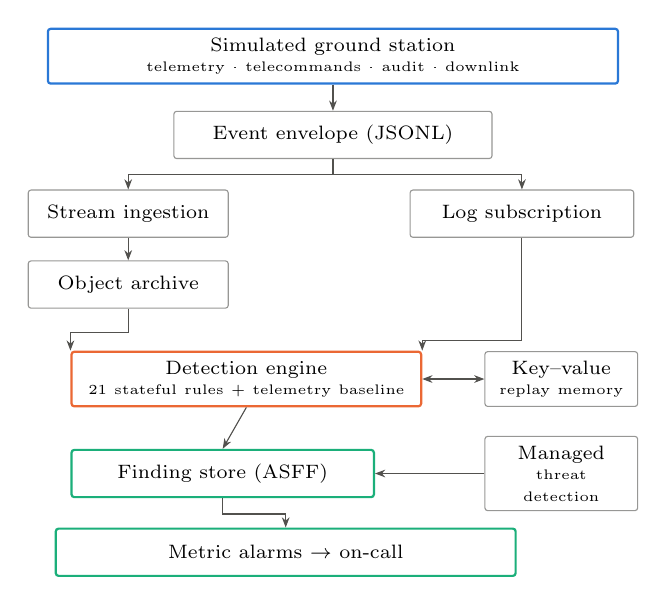
\begin{tikzpicture}[
  x=1mm, y=1mm,
  font=\scriptsize,
  box/.style={draw=vizink!60, rounded corners=1pt, align=center,
              inner sep=1.2mm, minimum height=6mm, fill=white},
  src/.style={box, draw=vizblue, thick},
  det/.style={box, draw=vizorange, thick},
  sink/.style={box, draw=vizaqua, thick},
  arr/.style={-{Stealth[length=1.3mm]}, draw=vizink, line width=0.4pt},
  arr2/.style={{Stealth[length=1.3mm]}-{Stealth[length=1.3mm]}, draw=vizink, line width=0.4pt}
]
\node[src, text width=70mm] (sim) at (41, 0)
  {Simulated ground station\\[-0.3mm]
   \tiny telemetry \textperiodcentered\ telecommands \textperiodcentered\ audit \textperiodcentered\ downlink};
\node[box, text width=38mm] (bus) at (41, -10) {Event envelope (JSONL)};
\node[box, text width=23mm] (kin) at (15, -20) {Stream ingestion};
\node[box, text width=26mm] (cwl) at (65, -20) {Log subscription};
\node[box, text width=23mm] (s3)  at (15, -29) {Object archive};
\node[det, text width=42mm] (eng) at (30, -41)
  {Detection engine\\[-0.3mm]
   \tiny \expRuleCount{} stateful rules $+$ telemetry baseline};
\node[box, text width=17mm] (ddb) at (70, -41) {Key--value\\[-0.3mm]\tiny replay memory};
\node[sink, text width=36mm] (sh)  at (27, -53) {Finding store (ASFF)};
\node[box, text width=17mm] (gd)  at (70, -53) {Managed\\[-0.3mm]\tiny threat detection};
\node[sink, text width=56mm] (ops) at (35, -63) {Metric alarms $\rightarrow$ on-call};

\draw[arr] (sim) -- (bus);
\draw[arr] (bus.south) -- ++(0,-2) -| (kin.north);
\draw[arr] (bus.south) -- ++(0,-2) -| (cwl.north);
\draw[arr] (kin) -- (s3);
\draw[arr] (s3.south) -- ++(0,-3) -| (eng.north west);
\draw[arr] (cwl.south) -- ++(0,-13) -| (eng.north east);
\draw[arr2] (ddb) -- (eng);
\draw[arr] (eng.south) -- (sh.north);
\draw[arr] (gd) -- (sh);
\draw[arr] (sh.south) -- ++(0,-2) -| (ops.north);
\end{tikzpicture}
\caption{Pipeline. The detection engine is the same object offline, under test
and in the cloud. Managed threat-detection findings are re-scored against the
mission asset inventory before entering the same queue.}
\label{fig:arch}
\end{figure}

\subsection{Event envelope and rule engine}

All four planes share one envelope: an identifier, a type, a coordinated
universal time stamp, the station identifier, a plane-specific payload, and (in
the lab only) the ground-truth label. A single stream means a single consumer,
and the audit payload deliberately mirrors the field names of a real cloud
trail so that the identity rules run unchanged against production logs.

The engine consumes events in timestamp order and emits findings carrying a
severity, an ATT\&CK technique, the evidence that triggered them and a
remediation. Severities and thresholds live in a catalogue separate from the
logic, so an operator can retune without a code deployment. State is bounded by
time rather than by event count. Three horizons appear: failed-login,
command-rate and anomaly-streak state over seconds to minutes; last-login
geography per operator over an hour; and accepted sequence counters and
authentication tags over the full anti-replay window of 24~hours.

Only the last horizon must be globally consistent. A replayed frame was
accepted hours earlier, quite possibly by a different function invocation on a
different shard, so replay detection is the one rule that cannot be answered
from a single batch. The engine therefore addresses a \emph{replay memory}
interface --- a dictionary offline, and in the cloud a key--value table with a
time-to-live and a conditional write, which makes the deduplication race-free
without a lock.

\subsection{Telemetry baseline}
\label{sec:model}

Let $x \in \mathbb{R}^{d}$, $d = 7$, be the vector of housekeeping channels. We
fit a single robust Gaussian on telemetry from a run known to be clean.
Location and scale are estimated per channel by the median and the normalised
median absolute deviation~\cite{rousseeuw1993mad}, so that the few outliers any
real archive contains do not drag the baseline:
\begin{equation}
\hat{\mu}_j = \operatorname{med}(x_j), \quad
\hat{\sigma}_j = 1.4826 \cdot \operatorname{med}\!\left(|x_j - \hat{\mu}_j|\right).
\end{equation}
Channels are standardised, $z = (x - \hat{\mu}) \oslash \hat{\sigma}$, and the
sample covariance $S$ of $z$ is shrunk towards its diagonal in the spirit
of~\cite{ledoit2004wellconditioned} with a fixed intensity $\lambda = 0.15$, so
that the inverse remains well conditioned on short baselines:
$\tilde{S} = (1 - \lambda) S + \lambda \operatorname{diag}(S)$. The anomaly
score of a sample is its squared Mahalanobis
distance~\cite{mahalanobis1936},
\begin{equation}
s(x) = z^{\top} \tilde{S}^{-1} z,
\label{eq:score}
\end{equation}
and the detection threshold $\tau$ is the empirical $q$-quantile of $s$ over
the training run, with $q = 0.999$ throughout. A finding is raised only after
$k = 3$ consecutive samples exceed $\tau$; Section~\ref{sec:results} shows that
this streak requirement is what converts a non-zero per-sample false-positive
rate into zero false alerts.

Three properties matter more than accuracy here. The model fits in
milliseconds, serialises to a \expModelKb~KB object that a serverless function
loads without a machine-learning layer, and decomposes: the per-channel
contributions to~\eqref{eq:score} are available for free, so a finding can name
the channels that moved. An analyst at 03:00 needs that more than a
fractionally better score, and Section~\ref{sec:results} shows the fractionally
better score was not on offer anyway.

\section{Implementation}
\label{sec:impl}

The simulated spacecraft is a 95-minute low-Earth orbit with a 35\% eclipse
fraction and an 11-minute contact window per orbit. The bus model is small but
deliberately \emph{coupled}: illumination drives the power budget, the power
budget and eclipse state drive the thermal channels, and transmit duty and slew
rate drive the amplifier temperature and the link margin. Coupling is what makes
RQ3 meaningful --- an adversary who moves one channel while leaving the others
untouched breaks the relationships long before breaking any single limit. The
station drives that model at a 30-second cadence and adds the three
ground-segment planes: shift handovers produce console sign-ins (service
identities federate through role assumption instead), contact windows produce
telecommands authenticated with a keyed tag over a canonical serialisation plus
a monotonic sequence counter, and each pass ends with a payload downlink.

Attacks are applied \emph{after} the nominal run, so "normal" is defined in one
place. Each injector receives the timeline and a context object, and returns the
timeline with its events inserted or mutated and labelled. Injectors therefore
compose --- the credential stage registers the hijacked session that the
tampering and exfiltration stages reuse, which produces genuine cross-plane
correlation rather than five independent incidents --- and because injection is
a transformation of a clean timeline, the same seed yields the same corpus byte
for byte.

The deployed pipeline maps each stage to a managed service: stream ingestion
partitioned by station, continuous archival to compressed object storage, the
engine in a serverless function with partial-batch failure reporting, the replay
memory in a key--value table with conditional writes and a time-to-live, the
identity plane from a cloud audit trail carrying both management and
object-level events, a managed threat-detection service re-scored by a second
function against the mission asset inventory, and findings in a single store in
a standard format~\cite{asff}.

Three defects appeared only once that cloud path was exercised against emulated
services, each a silent failure of the kind a simulation-only evaluation never
surfaces. The log-ingestion interface rejects events older than 14~days
\emph{inside a successful response}, so the reproducible corpus, whose
timestamps are fixed for determinism, vanished into an empty log group with a
zero exit code. Declaring advanced event selectors on the audit trail
\emph{replaces} the default management-event selector, so a data-events-only
configuration would have recorded no sign-ins or credential creations at all,
silently disabling the entire identity rule family. And the stream-to-function
mapping advertises partial-batch failure reporting, but a handler that does not
return the failed record identifiers makes one malformed record fail and retry
an entire 200-record batch. All three are fixed and covered by regression
tests.

\section{Experimental Methodology}
\label{sec:method}

\subsection{Corpus and protocol}

Table~\ref{tab:corpus} describes one \expSimHours-hour run. Telemetry dominates
by construction, at one sample every 30~seconds; the identity and downlink
planes are sparse, which is exactly the regime in which a per-event
false-positive rate matters. The label distribution is uneven and we do not
smooth it: \texttt{replay} and \texttt{exfiltration} label single-digit numbers
of events, while \texttt{anomalous\_behavior} labels several hundred telemetry
samples because the drift it injects persists for hours. Aggregate recall would
therefore be dominated by one scenario, so we report recall per scenario
throughout and never average it.

% Generated by paper/experiments.py -- do not edit by hand.
\begin{table}[t]
\caption{One 24-hour corpus: events by plane, and events carrying each attack label. Labelled events overlap the planes they occur in.}
\label{tab:corpus}
\centering
\begin{tabular}{@{}lrr@{}}
\toprule
 & \textbf{Events} & \textbf{\%} \\
\midrule
\multicolumn{3}{@{}l}{\emph{Evidence plane}} \\
\texttt{telemetry} & 2880 & 80.4 \\
\texttt{telecommand} & 583 & 16.3 \\
\texttt{audit} & 102 & 2.8 \\
\texttt{downlink} & 19 & 0.5 \\
\midrule
\multicolumn{3}{@{}l}{\emph{Attack label}} \\
\texttt{credential\_compromise} & 11 & 0.3 \\
\texttt{command\_tampering} & 43 & 1.2 \\
\texttt{replay} & 8 & 0.2 \\
\texttt{anomalous\_behavior} & 404 & 11.3 \\
\texttt{exfiltration} & 7 & 0.2 \\
\midrule
Benign & 3111 & 86.8 \\
\textbf{Total} & \textbf{3584} & \textbf{100.0} \\
\bottomrule
\end{tabular}
\end{table}


We run \expNumSeeds{} independent trials. Trial $i$ fits the telemetry baseline
on a clean \expSimHours-hour run generated with seed $i + 10^{4}$, then detects
on an attacked run generated with seed $i$. Training and evaluation data are
therefore disjoint and independently generated, and no attacked sample ever
reaches the model. All trials use the same rule catalogue and the same
$q = 0.999$ threshold quantile; nothing is tuned per trial or per scenario. All
experiments run single-threaded, and the artefact's result record stores the
library versions and platform string alongside every number reported here.

\subsection{Metrics, ablation and reference detectors}

A finding is a \emph{true positive} when the event it names carries an attack
label, and a \emph{false positive} otherwise. We report the \emph{detection
rate} (the fraction of trials in which a scenario produced at least one true
positive --- the question an operator asks); \emph{event-level recall} (within a
scenario, the fraction of its labelled events that produced at least one finding
--- the stricter question, and the one where a persistent scenario can be
"detected" while most of its events go unflagged); \emph{precision} and the
\emph{false-positive rate}, the latter over benign events rather than over
findings, so that it is comparable across scenarios of different sizes; and
\emph{mean time to detect} (MTTD), the interval between a scenario's first
labelled event and the first finding attributable to it.

We evaluate three configurations: \emph{rules only} (the catalogue with the
model-driven rule removed), \emph{model only} (that rule alone), and \emph{rules
$+$ model}. For RQ2 and RQ3 the model is compared against the two alternatives a
real mission already has. The first is the \emph{interface-control limits}: the
spacecraft's own red lines, encoded as a rule. This is the deployed status quo,
and the only honest comparison for whether a learned baseline earns its place.
The second is the \emph{best single channel}: a per-channel detector that
already knows the robust centre and scale of every channel and takes the largest
absolute standardised deviation, $u(x) = \max_j |z_j|$, thresholded at the same
training quantile. This is intentionally the strongest univariate strawman ---
it is given everything the multivariate model has except the covariance.

\subsection{The phase-swap probe}
\label{sec:probe}

The drift injected by \texttt{anomalous\_behavior} pushes several channels well
outside their own robust scale, which means it is detectable marginally and
cannot separate "multivariate" from "well-calibrated univariate". To test the
design claim directly we construct a probe that preserves every marginal exactly
while destroying the joint structure. In a clean run, each telemetry vector in a
\expSwapWindowMin-minute window is replaced by the vector observed exactly half
an orbit earlier, channel for channel. Every individual value is one the
spacecraft genuinely produced and lies inside its own learned marginal
distribution; the \emph{combination} --- eclipse-era power draw beside
sunlit-era temperatures --- is physically impossible. Orbit phase is not among
the model's features, so the substitution is invisible to any per-channel test
by construction, and detectable only by a model of the relationships between
channels.

The probe also models a real technique: replaying recorded housekeeping frames
to mask a fault or the effect of a malicious command. We keep it as a controlled
probe rather than a sixth deployed scenario so that the headline effectiveness
numbers describe the shipped system.

\section{Results}
\label{sec:results}

\subsection{RQ1: Effectiveness}

Table~\ref{tab:effectiveness} and Fig.~\ref{fig:ablation} give the main result.
All five scenarios are detected in all \expNumSeeds{} trials, at a precision of
$\expPrecision \pm \expPrecisionSD$ and a false-positive rate of
\expFprOverall\% of benign events. The four scenarios that leave discrete
evidence --- a forged tag, a reused counter, a policy attachment, a transfer to
an unapproved destination --- reach event-level recall of $1.00$ with zero
variance and an MTTD of $0$~seconds, because the first event of the scenario is
itself the violation.

% Generated by paper/experiments.py -- do not edit by hand.
\begin{table}[t]
\caption{Effectiveness over 20 independent trials. Detection rate is the percentage of trials in which the scenario produced at least one finding; recall is per labelled event. The last two columns give recall for the ablated configurations.}
\label{tab:effectiveness}
\centering
\begin{tabular}{@{}lrcrrr@{}}
\toprule
 & \textbf{Det.} & \textbf{Recall} & \multicolumn{2}{c}{\textbf{Recall (ablated)}} & \textbf{MTTD} \\
\cmidrule(lr){4-5}
\textbf{Scenario} & \textbf{\%} & \textbf{rules\,+\,model} & \textbf{rules} & \textbf{model} & \textbf{(s)} \\
\midrule
\texttt{credential\_compromise} & 100 & $0.82 \pm 0.00$ & 0.82 & 0.00 & 18 \\
\texttt{command\_tampering} & 100 & $1.00 \pm 0.00$ & 1.00 & 0.00 & 0 \\
\texttt{replay} & 100 & $1.00 \pm 0.00$ & 1.00 & 0.00 & 0 \\
\texttt{anomalous\_behavior} & 100 & $0.97 \pm 0.00$ & 0.19 & 0.97 & 342 \\
\texttt{exfiltration} & 100 & $1.00 \pm 0.00$ & 1.00 & 0.00 & 0 \\
\midrule
\multicolumn{6}{@{}l}{Precision (rules\,+\,model): $0.997 \pm 0.002$} \\
\multicolumn{6}{@{}l}{False positives: 0.06\% of benign events} \\
\bottomrule
\end{tabular}
\end{table}


\begin{figure*}[t]
\centering

\includegraphics{ablation.pdf}
\caption{Event-level recall by scenario and configuration, mean over
\expNumSeeds{} trials with standard-deviation bars. Absent bars are zero. The
rule catalogue and the learned baseline are complementary rather than
overlapping: neither configuration alone covers the corpus.}
\label{fig:ablation}
\end{figure*}

The ablation shows the two halves are complementary and non-overlapping. The
model alone detects nothing outside the telemetry plane --- it has nothing to
say about a forged authentication tag --- and the rules alone reach only
\expRecAnomalyRules{} recall on the behavioural drift. Together they cover the
corpus. The model configuration attains a precision of \expPrecisionMl{} with
zero false positives in any trial, which is the streak requirement of
Section~\ref{sec:model} doing its work: the per-sample false-positive rate at
the operating point is \expFprTelemetryOp\%, but isolated exceedances never
survive three consecutive samples.

The residual false positives are concentrated in two rules and are worth naming
rather than rounding away. The impossible-travel rule fires
\expFpAuthPerTrial{} times per trial, always on the \emph{legitimate} operator
sign-in that follows the attacker's --- correct behaviour that a label-based
metric is obliged to count as an error. The command-rate rule fires
\expFpRatePerTrial{} times in the trials where it fires at all, on nominal
bursts that cross a per-operator ceiling set too tightly. The first is a metric
artefact; the second is a genuine tuning defect.

\subsection{RQ2: What the baseline adds over spacecraft limits}

This is the comparison that matters operationally, because the limit check is
what a mission already runs. Across trials, the learned baseline raises a
finding
$\expLeadMean \pm \expLeadSD$~minutes before the first limit violation (range
\expLeadMin--\expLeadMax~minutes, and in no trial did the limit fire first).
Event-level recall for the drift rises from \expRecAnomalyRules{} to
\expRecAnomalousBehavior{}, and MTTD falls from \expMttdAnomalyRules{} to
\expMttdAnomalyAll{}~minutes.

The interpretation is narrow and we state it narrowly: a limit check tells an
operator the spacecraft is \emph{already} outside its design envelope, whereas
the baseline tells them it is heading there. Forty minutes is the difference
between diagnosing a degradation and reacting to an alarm. It is not evidence
that the model is a good anomaly detector in general --- only that it is a
better early indicator than a red line.

\subsection{RQ3: Multivariate versus univariate --- two negative results}

\emph{On the injected drift, the covariance buys nothing.} On the telemetry
plane of the attacked runs, over \expNumSeeds{} trials, the multivariate
detector achieves an area under the receiver operating characteristic curve of
$\expAucMulti \pm \expAucMultiSD$ and the best single channel
$\expAucUni \pm \expAucUniSD$. The univariate detector is marginally
\emph{better}, the gap is smaller than the between-trial spread, and over the
full range the two curves are visually indistinguishable.
The rationale we designed the model around --- that correlation is what makes a
sub-threshold attack visible --- is not supported for this attack.

The explanation is in the attack, not the model. The injected drift moves the
slew rate, bus current and amplifier temperature several robust standard
deviations from their own centres, so each channel is individually anomalous and
a per-channel test suffices. A fair reading is that our behavioural scenario is
easier than intended, and that the experiment does not test the claim.

\emph{On an attack that isolates the joint structure, both detectors fail.} The
phase-swap probe of Section~\ref{sec:probe} does test it, and the result is
worse than inconclusive. Fig.~\ref{fig:phaseswap} shows why: the swapped vectors
do not merely fail to exceed the threshold, they score \emph{lower} than nominal
telemetry --- median squared distance \expSwapMedianSwapped{} against
\expSwapMedianNormal{} for nominal samples. Both detectors are below chance
($\expAucSwapMulti \pm \expAucSwapMultiSD$ multivariate,
$\expAucSwapUni \pm \expAucSwapUniSD$ univariate) and the attack is flagged in
only \expSwapDetectedMulti{} of \expNumSeeds{} trials.

\begin{figure}[t]
\centering

\includegraphics{phaseswap.pdf}
\caption{Score distributions under the phase-swap probe. Replayed housekeeping
frames from half an orbit earlier sit \emph{inside} --- indeed below --- the
nominal distribution, because orbit phase is marginalised away by a baseline
fitted over a whole orbit. Texture is redundant with colour for grayscale
printing.}
\label{fig:phaseswap}
\end{figure}

This is a structural limitation, not a tuning problem, and no threshold fixes
it. A single Gaussian fitted over an entire orbit learns the \emph{average}
relationship between channels, marginalising over the phase; any vector that
occurred at any phase is therefore in-distribution. That the swapped samples
score below the median follows: mid-orbit values are denser than the extremes
the true samples occupy. An adversary who replays valid old telemetry hides
inside the learned baseline, and makes the spacecraft look healthier than it is.
Because the failure is below chance it is also \emph{exploitable}: the same
replay drives the anomaly score down while a fault progresses.

The fix is to condition on phase rather than to marginalise it: model the
residual from a phase-dependent expectation, or fit a mixture indexed by orbit
phase, including phase as an explicit conditioning variable. We report the
failure rather than implementing the fix here, because the probe is the
contribution --- it is a cheap, reusable test that any spacecraft telemetry
detector can be subjected to, and we would expect several published detectors to
fail it. We think the implication generalises: any detector that fits a
phase-marginal distribution over a periodic system inherits the same blind spot,
including detectors considerably more sophisticated than
ours~\cite{hundman2018lstm,yairi2017datadriven}, unless they condition on phase
explicitly.

\subsection{RQ4: How much clean telemetry the baseline needs}

Fig.~\ref{fig:baseline} sweeps the size of the training window. The finding is a
sharp threshold rather than a gradual improvement: fitting on one hour yields a
telemetry false-positive rate of \expFprOneHour\%, reaching \expFprFullDay\%
only once the window covers a full \expSimHours{} hours. Discrimination improves
marginally across the sweep (area under the curve \expAucBaselineMin{} to
\expAucBaselineMax{}) and the true-positive rate declines slightly as the
threshold rises, so neither explains the collapse.

\begin{figure}[t]
\centering

\includegraphics{baseline.pdf}
\caption{Baseline-size sensitivity. Upper panel: telemetry false-positive rate
at the deployed operating point. Lower panel: area under the curve and
true-positive rate. The false-positive rate collapses only when the training
window covers a full diurnal cycle; discrimination barely changes.}
\label{fig:baseline}
\end{figure}

The cause is coverage, not sample size. A window shorter than the orbital and
diurnal cycle observes only part of the state space --- some eclipse fractions,
some contact geometries, some thermal regimes --- so the quantile threshold is
calibrated against a distribution the deployed model will not see. The
operational rule this implies is concrete: a baseline must span at least one
full cycle of every periodicity the mission has, and a detector that reported
only the area under the curve would have concluded, wrongly, that one hour of
data is nearly as good as a day.

\subsection{RQ5: Cost and alert volume}

The engine processes \expThroughputMl{} events per second with the model enabled
(\expUsPerEventMl~$\mu$s per event) and \expThroughputRules{} without it;
fitting the baseline on a day of telemetry takes \expFitSeconds{}~s and produces
a \expModelKb~KB model. At a 30-second telemetry cadence, one core is
approximately five orders of magnitude faster than one station requires, so the
detection cost is not the constraint --- transport and storage are.

The analyst-facing load is a different matter. The mean of \expFindingsMean{}
findings per simulated day is a misleading summary: the load is extremely
bursty, with nothing for twenty hours and a peak of roughly
\expAlertPeakHour{} findings in a single hour, of which \expCriticalPerDay{} per
day are critical. Aggregate false-positive rates say little about whether a
queue is workable, and the base-rate fallacy~\cite{axelsson2000baserate} applies
with full force at these volumes. The practical mitigation in our design is
severity discipline plus correlation: critical findings page, and the chains in
Table~\ref{tab:paths} mean an operator sees one incident rather than four
unrelated alerts.

\section{Discussion and Limitations}
\label{sec:limitations}

\subsection{Rules and models do different jobs}

The ablation makes a point easy to lose in a field enthusiastic about learned
detection: the four highest-impact scenarios --- forged commands, replay,
privilege escalation, exfiltration --- are caught by deterministic rules,
immediately, with no variance and no training data, because the mission has an
explicit policy to state (a tag must verify; a counter must not repeat; a role
may not issue this opcode) and a rule is the natural expression of a policy.
Learned detection earns its place only where no policy exists to state:
behaviour legal at every instant and wrong in aggregate. Our two negative
results point the same way --- the marginals carry most of the signal a static
baseline can extract, and the joint structure it learns is too coarse to catch
an adversary who respects them. Separately, the three silent failures in
Section~\ref{sec:impl} share a shape: the cloud interface accepted the request,
returned success, and discarded the data or the configuration intent. A
detection pipeline is precisely the kind of system in which that is invisible,
because an empty log group and a quiet queue look identical to a quiet day.

\subsection{Threats to validity}

\emph{The corpus is synthetic.} This is the dominant threat and we do not
minimise it. Our spacecraft model is a sine-wave illumination profile with
first-order thermal lags; real housekeeping telemetry has instrument
nonlinearity, sensor faults, seasonal beta-angle drift and operator
idiosyncrasy that we do not reproduce, so absolute numbers should be read as
properties of this corpus rather than of a mission. The comparative and
structural findings --- the rules/model complementarity, the ordering of lead
times, the phase-swap blindness, the coverage threshold --- depend on the
\emph{structure} of the data rather than its fidelity, and we expect them to
transfer; the precision figure does not.

\emph{Attacks are injected, not executed}, and the adversary is non-adaptive:
it does not observe the detector and adjust, which is the weakest assumption in
any static evaluation of this kind~\cite{sommer2010closedworld}. The phase-swap
probe is our one concession to an adaptive adversary, and it succeeded. Recall
is also per event, so a scenario labelling 404 events and one labelling 7 are
not comparable, and the impossible-travel false positive in
Section~\ref{sec:results} is correct detector behaviour scored as an error; we
report per-scenario numbers to keep this visible rather than resolving it.

\emph{Scope.} One station, one spacecraft, one region; cross-station
correlation is a stronger signal than either station alone and we do not
evaluate it. The cloud evaluation is emulated in process, so it cannot surface
authorisation-policy mistakes, service quotas or eventual consistency, and the
infrastructure code has not been applied against a live account --- the
deployed pipeline's cost and latency are unmeasured. We also evaluate one
baseline family; isolation forests~\cite{liu2008isolation}, sequence
models~\cite{hundman2018lstm} and probabilistic
clustering~\cite{yairi2017datadriven} are the obvious comparisons and are left
to future work, and the model sits behind a score-and-threshold interface so
they can be substituted and scored on the same labels.

\section{Related Work}

\emph{Space systems security.} Pavur and Martinovic surveyed the field and
argued that its central problem is the absence of reproducible artefacts and
shared testbeds~\cite{pavur2020sok}; this paper responds to that argument for
one part of the system. Pavur et al.\ demonstrated practical interception of
operational maritime satellite links~\cite{pavur2020vsat}, and Willbold et al.\
analysed real satellite firmware and found systematic absence of authentication
on the commanding path~\cite{willbold2023space}.
Falco~\cite{falco2019principles} and Manulis et
al.~\cite{manulis2021newspace} set out security principles for space systems
and for the commercial segment; SPARTA~\cite{sparta} and ATT\&CK~\cite{attack}
provide the taxonomies we map to, and the commanding model follows the CCSDS
telecommand protocol~\cite{ccsds232} and its security layer~\cite{ccsds355}.
Our focus differs in being the ground segment's cloud footprint, and in being
evaluated against labels rather than argued.

\emph{Telemetry anomaly detection and evaluation methodology.} Detecting faults
in housekeeping telemetry is mature: Hundman et al.\ applied recurrent networks
with nonparametric dynamic thresholding to spacecraft
channels~\cite{hundman2018lstm}, Yairi et al.\ combined probabilistic
clustering with dimensionality reduction~\cite{yairi2017datadriven}, and
Chandola et al.\ survey the wider area~\cite{chandola2009survey}. That
literature targets \emph{faults}, and its evaluations assume anomalies are not
adversarially chosen; our phase-swap result suggests the assumption is
load-bearing, because a fault will not respect the marginals and an adversary
will. On the reporting side, Sommer and Paxson's critique of machine learning
for intrusion detection~\cite{sommer2010closedworld} and Axelsson's base-rate
analysis~\cite{axelsson2000baserate} shape how we present results --- per
scenario rather than aggregate, false positives over benign events, and alert
volume as a first-class result. Ring et al.\ survey the network intrusion
detection datasets~\cite{ring2019datasets} whose absence here motivated the
corpus, and automated adversary emulation in the style of
CALDERA~\cite{applebaum2016caldera} informed the composing-injector design.

\section{Conclusion}

We built an open, labelled testbed for detecting attacks on satellite ground
stations, and a cloud-native pipeline that detects five emulated scenarios in
every one of \expNumSeeds{} trials at $\expPrecision \pm \expPrecisionSD$
precision. The result we consider most useful is not that number. It is that
deterministic policy rules, not learned detection, carry the high-impact
scenarios; that the learned baseline earns its place on exactly one of the five,
where it buys $\expLeadMean$~minutes over the spacecraft's own limits; that its
multivariate machinery does not outperform a well-calibrated per-channel
detector on that scenario; and that both are blind --- below chance --- to an
adversary who replays valid telemetry from a different orbit phase. The last
finding is structural, applies to any phase-marginal baseline, and is testable
in a few lines of code. The artefact is public, deterministic, and runs offline
in seconds, so each of these claims can be checked and, we hope, improved on.

\section*{Acknowledgments}

\textbf{Declaration of generative AI use.} In accordance with IEEE policy on
the use of artificial intelligence--generated text, the author declares that a
large language model (Anthropic Claude, accessed through the Claude Code
command-line interface) was used substantially in preparing this work: it
assisted in writing the simulator, the detection engine, the infrastructure
code and the experiment harness, and in drafting and translating this
manuscript. All experimental results were produced by executing the released
code, and the author reviewed and verified the content and takes full
responsibility for it.

\textbf{Ethical considerations.} No real ground station, spacecraft or
third-party system was touched. All telemetry, credentials and audit records are
synthetic; the cryptographic keys in the repository are lab constants, labelled
as such, and unsuitable for operational use. The attack scenarios describe
adversary behaviour at the level of detection engineering and contain no exploit
code and no vulnerability in any real product.

\bibliographystyle{IEEEtran}
\bibliography{refs}

\end{document}
